%%%%%%%%%%%%%%%%%%%%%%%%%%%%%%%%%%%%%%%%%
% Beamer Presentation
% LaTeX Template
% Version 1.0 (10/11/12)
%
% This template has been downloaded from:
% http://www.LaTeXTemplates.com
%
% License:
% CC BY-NC-SA 3.0 (http://creativecommons.org/licenses/by-nc-sa/3.0/)
%
%%%%%%%%%%%%%%%%%%%%%%%%%%%%%%%%%%%%%%%%%

%----------------------------------------------------------------------------------------
%	PACKAGES AND THEMES
%----------------------------------------------------------------------------------------

\documentclass{beamer}

\mode<presentation> {

% The Beamer class comes with a number of default slide themes
% which change the colors and layouts of slides. Below this is a list
% of all the themes, uncomment each in turn to see what they look like.

%\usetheme{default}
%\usetheme{AnnArbor}
%\usetheme{Antibes}
%\usetheme{Bergen}
%\usetheme{Berkeley}
%\usetheme{Berlin}
%\usetheme{Boadilla}
%\usetheme{CambridgeUS}
%\usetheme{Copenhagen}
%\usetheme{Darmstadt}
%\usetheme{Dresden}
%\usetheme{Frankfurt}
%\usetheme{Goettingen}
%\usetheme{Hannover}
%\usetheme{Ilmenau}
%\usetheme{JuanLesPins}
%\usetheme{Luebeck}
\usetheme{Madrid}
%\usetheme{Malmoe}
%\usetheme{Marburg}
%\usetheme{Montpellier}
%\usetheme{PaloAlto}
%\usetheme{Pittsburgh}
%\usetheme{Rochester}
%\usetheme{Singapore}
%\usetheme{Szeged}
%\usetheme{Warsaw}

% As well as themes, the Beamer class has a number of color themes
% for any slide theme. Uncomment each of these in turn to see how it
% changes the colors of your current slide theme.

%\usecolortheme{albatross}
%\usecolortheme{beaver}
%\usecolortheme{beetle}
%\usecolortheme{crane}
%\usecolortheme{dolphin}
%\usecolortheme{dove}
%\usecolortheme{fly}
%\usecolortheme{lily}
%\usecolortheme{orchid}
%\usecolortheme{rose}
%\usecolortheme{seagull}
%\usecolortheme{seahorse}
%\usecolortheme{whale}
%\usecolortheme{wolverine}

%\setbeamertemplate{footline} % To remove the footer line in all slides uncomment this line
%\setbeamertemplate{footline}[page number] % To replace the footer line in all slides with a simple slide count uncomment this line

%\setbeamertemplate{navigation symbols}{} % To remove the navigation symbols from the bottom of all slides uncomment this line
}

\usepackage{graphicx} % Allows including images
\usepackage{booktabs} % Allows the use of \toprule, \midrule and \bottomrule in tables

%----------------------------------------------------------------------------------------
%	TITLE PAGE
%----------------------------------------------------------------------------------------

\title[social and financial interactions]{Interplay between social and financial interactions in a crypto-currency } % The short title appears at the bottom of every slide, the full title is only on the title page

\author{\textbf{Nicolas Gensollen}, Matthieu Latapy} % Your name
\institute[LIP6] % Your institution as it will appear on the bottom of every slide, may be shorthand to save space
{
Laboratoire d'informatique de Paris 6 \\ % Your institution for the title page
\medskip
\textit{nicolas.gensollen@lip6.fr \\
\bigskip
MARAMI 2019 - Dijon - France} % Your email address
}
\bigskip
\date{November 6, 2019} % Date, can be changed to a custom date

\begin{document}

\begin{frame}
\titlepage % Print the title page as the first slide
\end{frame}

\begin{frame}
\frametitle{Overview} % Table of contents slide, comment this block out to remove it
\tableofcontents % Throughout your presentation, if you choose to use \section{} and \subsection{} commands, these will automatically be printed on this slide as an overview of your presentation
\end{frame}

%----------------------------------------------------------------------------------------
%	PRESENTATION SLIDES
%----------------------------------------------------------------------------------------


%------------------------------------------------
\section{Context} 
%------------------------------------------------

\begin{frame}
\Huge{\centerline{Context}}
\end{frame}


%------------------------------------------------
\subsection{Who are we?}
%------------------------------------------------

\begin{frame}
	\frametitle{\textbf{Who} we are and \textbf{what} we do}
	\only<1>{{\Large \textbf{The team}}}
	\onslide<2-3>{{\Large \textbf{Our main research topics}}}
	\only<2>{\\ \bigskip \textbf{Stream Graphs}}
	\only<3>{\\ \bigskip \textbf{Anomaly detection}}
	\begin{center}
		\only<1>{
		\begin{itemize}
			\item \textit{Complex Networks} team (LIP6).
			\item Internet measurements, random graphs, temporal networks
			\item Social network analysis, spreading phenomena, graph algorithms
		\end{itemize}
		\bigskip
		\begin{figure}
			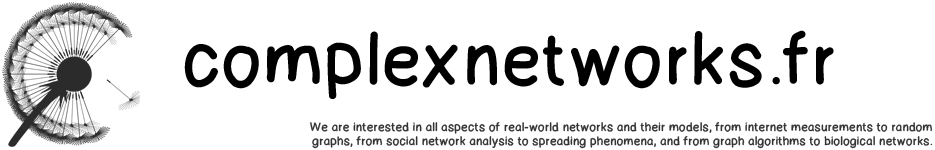
\includegraphics[width=\linewidth]{./figures/header}
		\end{figure}	
		}
		\only<2>{
		\bigskip
		\begin{figure}
			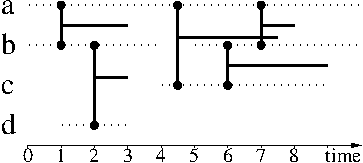
\includegraphics[width=.8\linewidth]{./figures/stream_graph}
		\end{figure}
		}
		\only<3>{
		\bigskip
		\begin{figure}
			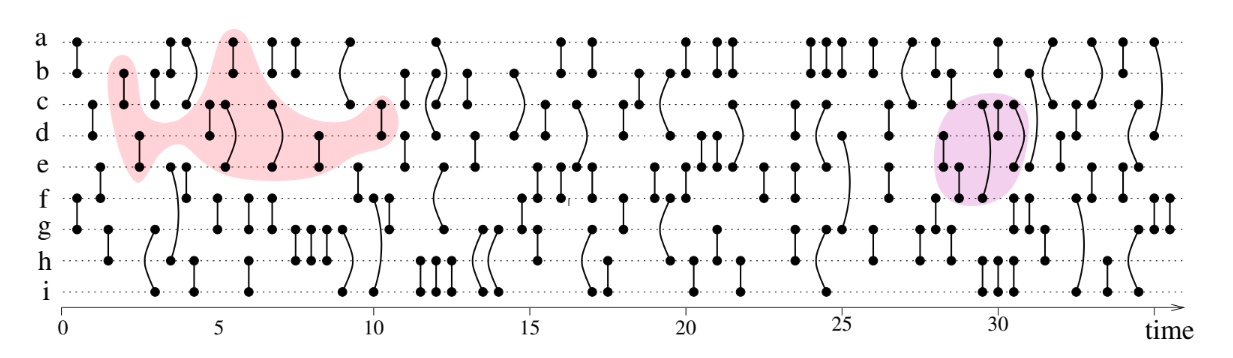
\includegraphics[width=\linewidth]{./figures/anomalie_detection}
		\end{figure}
		}
	\end{center}
\end{frame}


%------------------------------------------------
\subsection{The G1 crypto-currency}
%------------------------------------------------

\begin{frame}
	\frametitle{The G1 crypto-currency}
	\onslide<1->{\textbf{Enables transactions between members}}
	\medskip
	\onslide<2->{\\{\small A transaction $\left(t,u,v\right) \in \mathcal{T}$: \textit{Entity $u$ sends money to entity $v$ at time $t$}.}}
	\bigskip
	\only<3>{
	\begin{center}
		\begin{figure}
			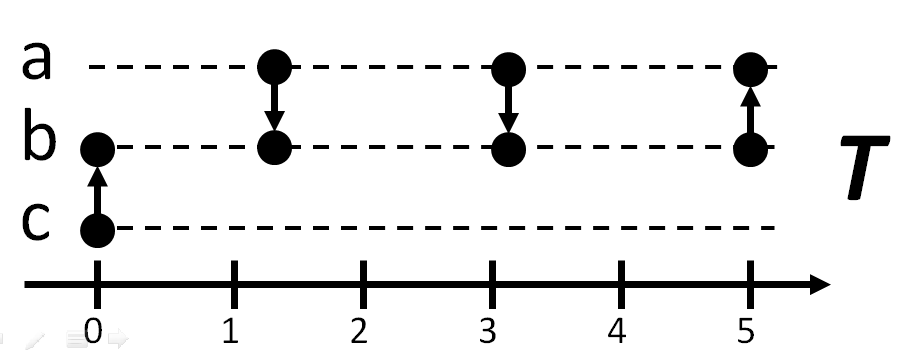
\includegraphics[width=\linewidth]{./figures/transaction}
		\end{figure}
	\end{center}}	
\end{frame}

%------------------------------------------------

\begin{frame}
	\frametitle{The G1 crypto-currency}
	\onslide<1->{\textbf{Identification of the members with a Web of Trust}}
	\medskip
	\onslide<2->{\\{\small A certification $\left(t,u,v\right) \in \mathcal{C}$: \textit{Member $u$ certifies identity of members $v$ at time $t$}.}}
	\bigskip
	\only<3>{
	\begin{center}
		\begin{figure}
			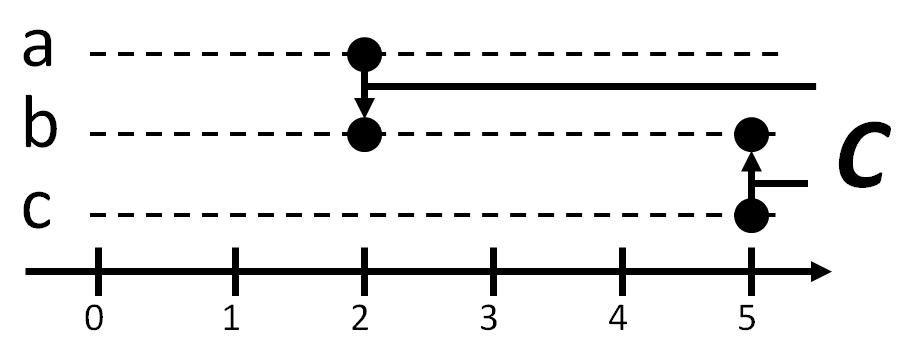
\includegraphics[width=\linewidth]{./figures/certification}
		\end{figure}
	\end{center}}	
\end{frame}

%------------------------------------------------

\begin{frame}
	\frametitle{Why is this great?}
	\textbf{{\footnotesize We have a dynamic network of social ties and financial transactions between identified human beings!}}
	\begin{center}
		\begin{figure}
			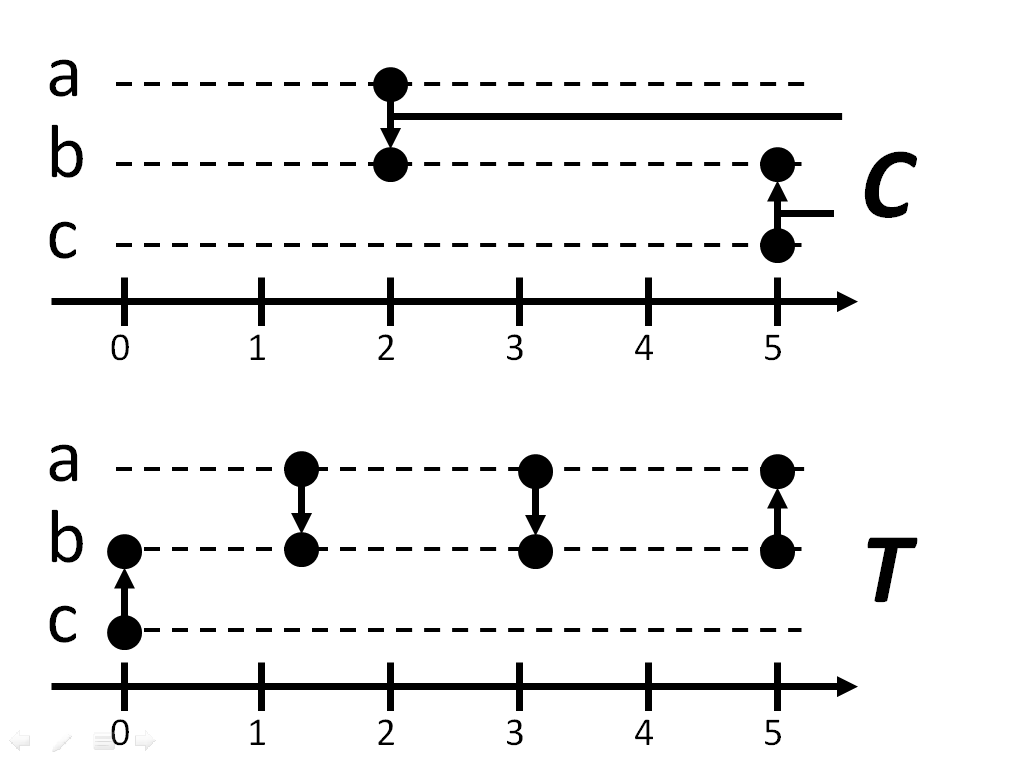
\includegraphics[width=.8\linewidth]{./figures/delta-t-0}
		\end{figure}
	\end{center}
\end{frame}


%------------------------------------------------
\subsection{Objectives of this work}
%------------------------------------------------

\begin{frame}
	\frametitle{Objectives of this work}
	\begin{itemize}
		\item<1-> Study the interplay between transactions and social ties
		\item<2-> Are my transaction partners the same
as my friends?
		\item<3-> Do transactions precede social ties or vice-versa?
		\item<4-> How do my friends exchange between them compared to my transaction partners?
		\item<5-> Are my friends and transaction partners more and more homogeneous over time?
		\item<6-> \textbf{Show how stream graphs can be used to gain insight on such questions}	 
	\end{itemize}
\end{frame}



%------------------------------------------------
\section{Approach}
%------------------------------------------------

\begin{frame}
	\Huge{\centerline{Approach}}
\end{frame}

%------------------------------------------------
\subsection{Data}
%------------------------------------------------

\begin{frame}
	\frametitle{What does the \textbf{data} look like?}
	\begin{itemize}
		\item<1-> Extract from the blockchain a stream of transactions $\mathcal{T}$ and a stream of certifications $\mathcal{C}$.
		\item<2-> A transaction $\left(t,u,v,a\right) \in \mathcal{T}$: \textit{Entity $u$ sends amount $a$ to entity $v$ at time $t$}.
		\item<3-> A certification $\left(t,u,v\right) \in \mathcal{C}$: \textit{Member $u$ certifies the identity of members $v$ at time $t$}.
	\end{itemize}
\end{frame}

%------------------------------------------------
\subsection{Stream Graphs}
%------------------------------------------------

\begin{frame}
	\frametitle{Approach}
	\only<1>{data: sequence of $\left(t,u,v\right)$}
	\only<2>{Aggregate interactions: lose structure}
	\only<3>{Aggregate time: lose dynamics/ordering}
	\only<4>{Other \textit{"in-between"} approaches also have drawbacks...}
	\only<5>{Solution: Model keeping both structure and time: \textbf{Stream Graphs}!}
	\begin{center}
		\begin{figure}
			\only<1>{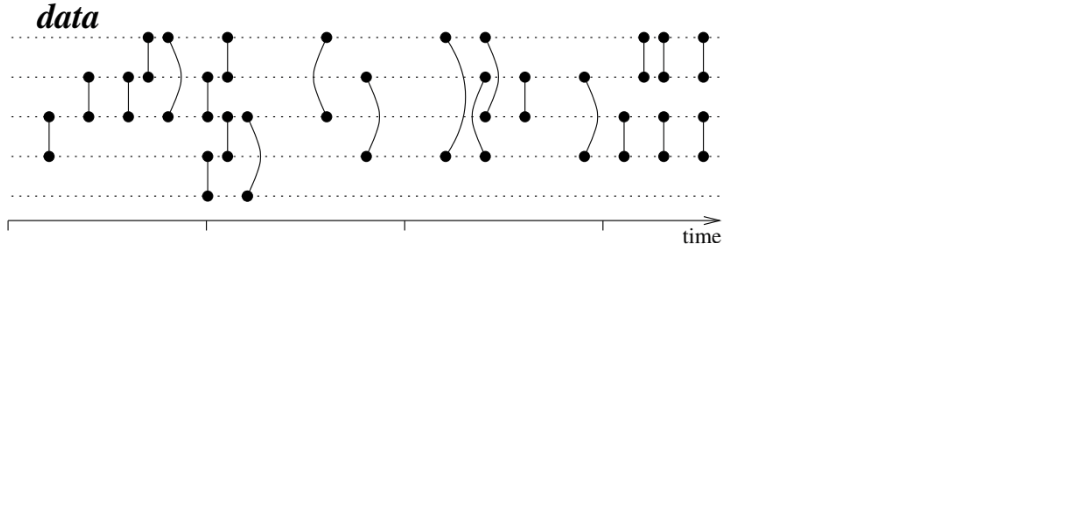
\includegraphics[width=\linewidth]{./figures/stream_graph_signal_stream_only.png}}
			\only<2>{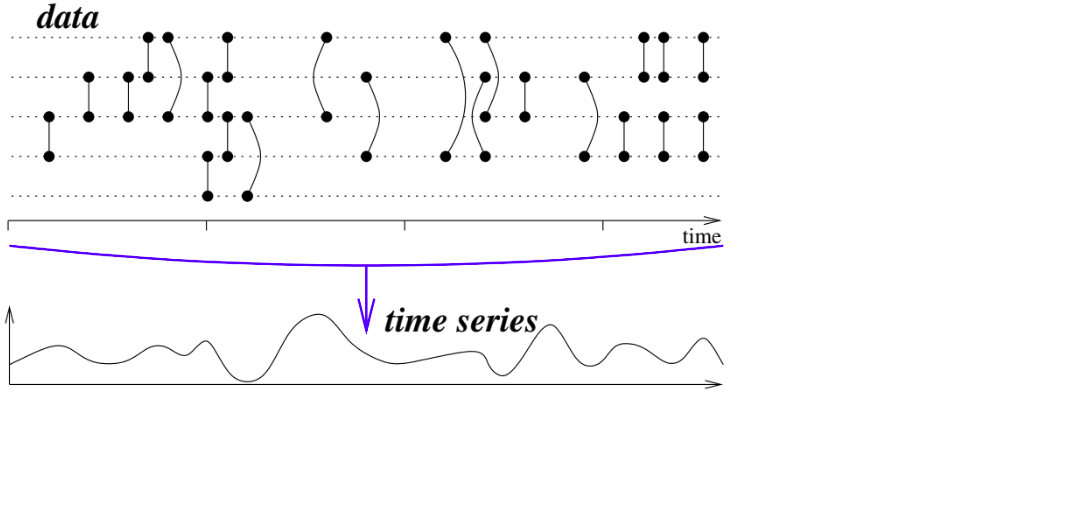
\includegraphics[width=\linewidth]{./figures/stream_graph_signal_signal_only.png}}
			\only<3>{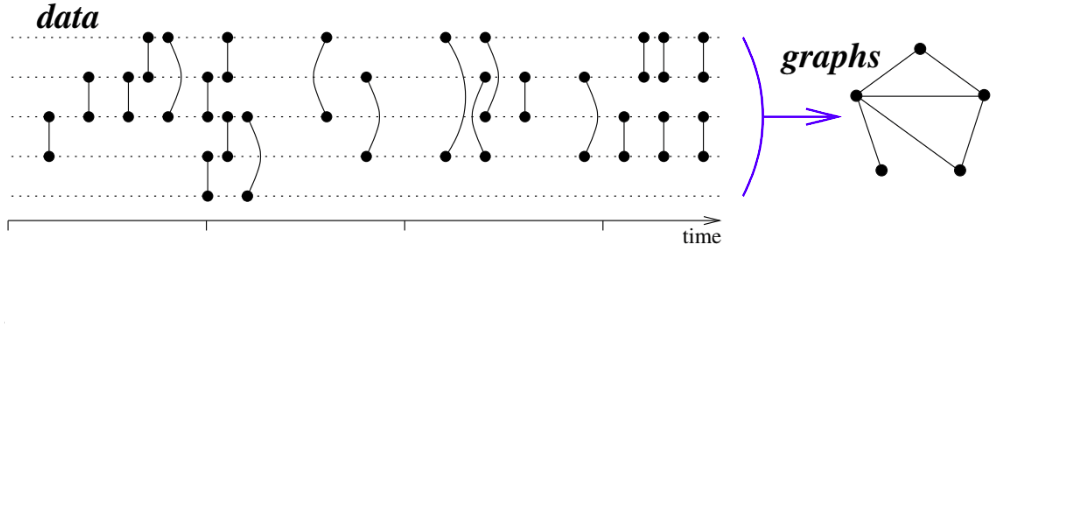
\includegraphics[width=\linewidth]{./figures/stream_graph_signal_graph_only.png}}
			\only<4>{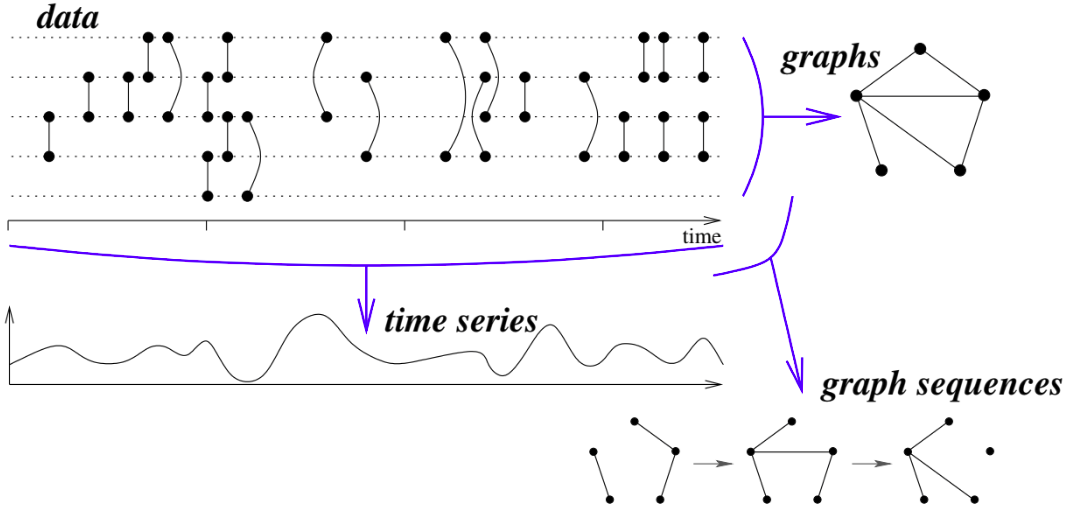
\includegraphics[width=\linewidth]{./figures/stream_graph_signal}}
			\only<5>{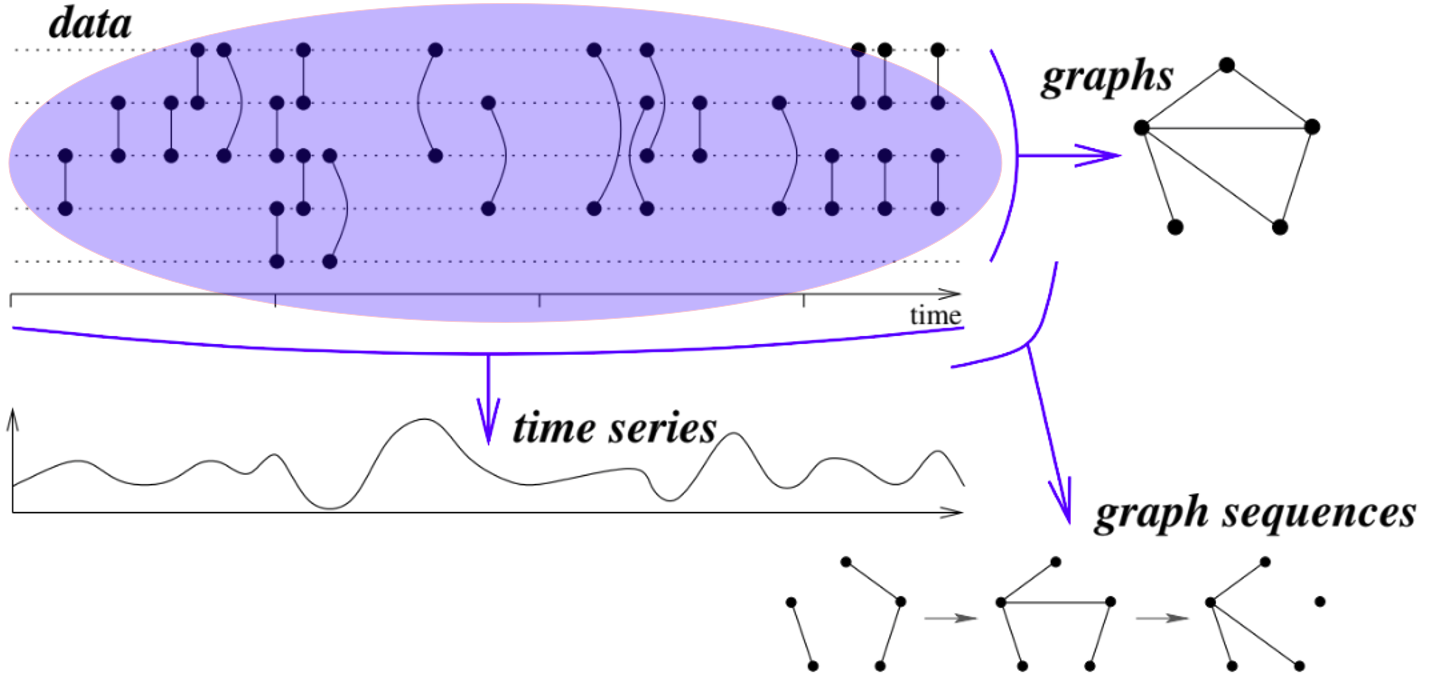
\includegraphics[width=\linewidth]{./figures/stream_graph_signal_final}}
		\end{figure}
	\end{center}
\end{frame}

%------------------------------------------------

\begin{frame}
	\frametitle{Stream Graphs}
	\begin{center}
		\only<1>{$ S = \left(T,V,W,E\right) $}
		\only<2>{$T$: Set of time instants}
		\only<3>{$V$: Set of nodes}
		\only<4>{$W \subseteq T \times V$: Set of temporal nodes}
		\only<5>{$E \subseteq T \times V \otimes V$: Set of link}
		\begin{figure}
			\only<1>{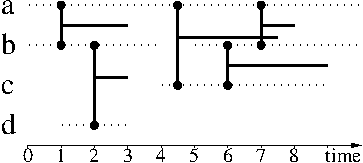
\includegraphics[width=.9\linewidth]{./figures/stream_graph}}
			\only<2>{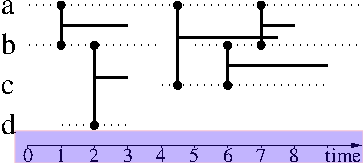
\includegraphics[width=.9\linewidth]{./figures/stream_graph_T}}
			\only<3>{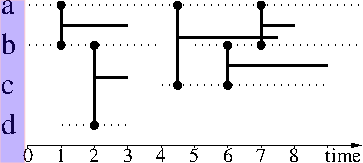
\includegraphics[width=.9\linewidth]{./figures/stream_graph_V}}
			\only<4>{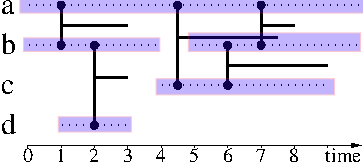
\includegraphics[width=.9\linewidth]{./figures/stream_graph_W}}
			\only<5>{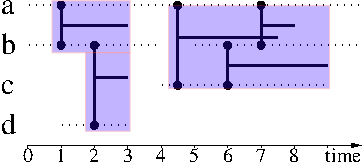
\includegraphics[width=.9\linewidth]{./figures/stream_graph_E}}
		\end{figure}
	\end{center}
\end{frame}

%------------------------------------------------

\begin{frame}
	\frametitle{Why is this useful?}	
	\begin{center}
		\begin{figure}
			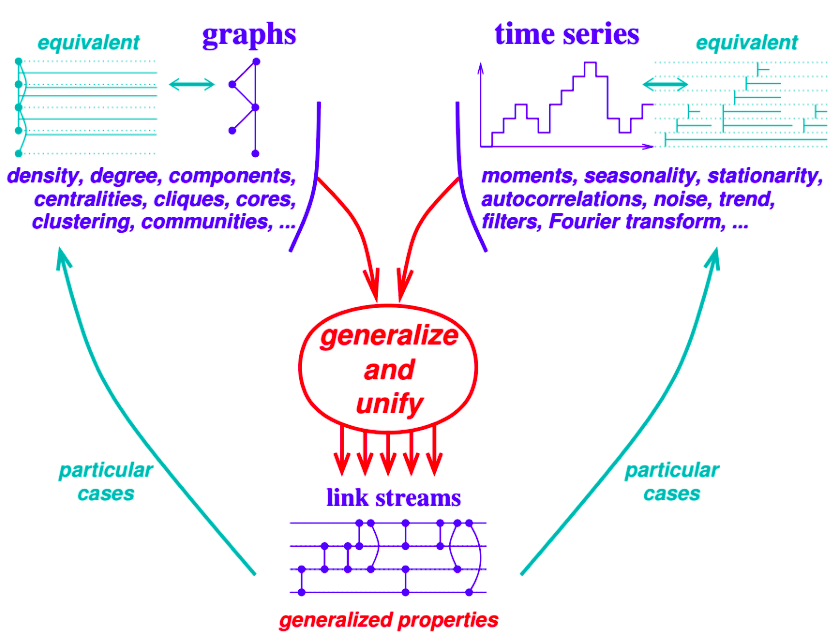
\includegraphics[width=.8\linewidth]{./figures/stream_unification}
		\end{figure}
	\end{center}
\end{frame}


%------------------------------------------------
\section{Results}
%------------------------------------------------

%------------------------------------------------
\subsection{Time between Transactions and Certifications}
%------------------------------------------------

\begin{frame}
	\Huge{\centerline{Results}}
\end{frame}

%------------------------------------------------

\begin{frame}
	\frametitle{Time between transactions and certifications - \textbf{Questions}}
	{\Large \textbf{Questions:}}
	\bigskip
	\begin{itemize}
		\item<1-> If $a$ and $b$ are certified, did/will they make transactions? 
		\medskip
		\item<2-> How much time separate the certification from the closest matching transaction?
		\medskip
		\item<3-> If $a$ and $b$ make a new transaction, are/will they certify?
		\medskip
		\item<4-> How much time separate the transaction from the closest matching certification?
	\end{itemize}
\end{frame}


%------------------------------------------------

\begin{frame}
	\frametitle{Time between transactions and certifications - \textbf{Method}}
	\begin{center}
		\begin{figure}
			\only<1>{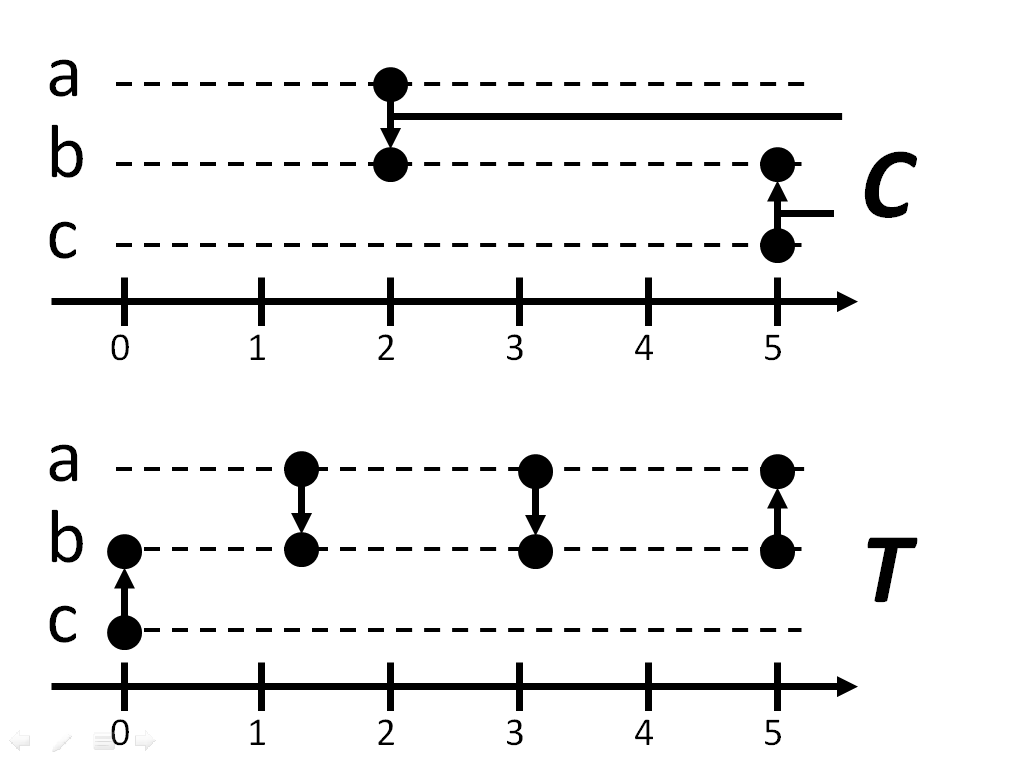
\includegraphics[width=.9\linewidth]{./figures/delta-t-0.png}}
			\only<2>{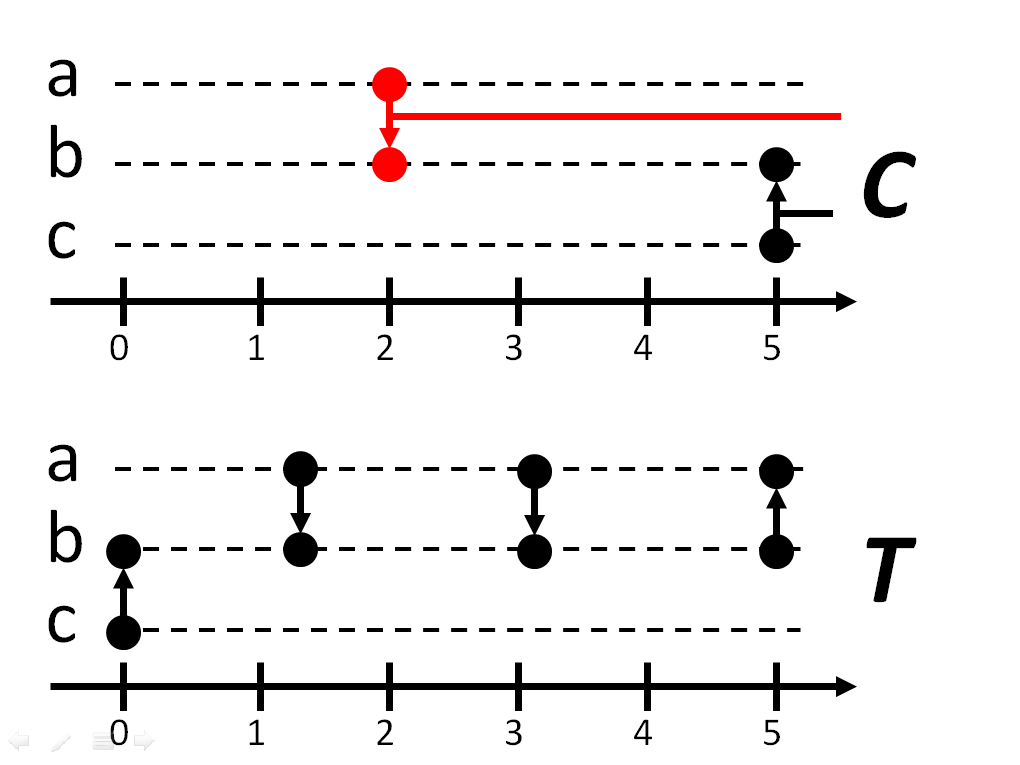
\includegraphics[width=.9\linewidth]{./figures/delta-t-1.png}}
			\only<3>{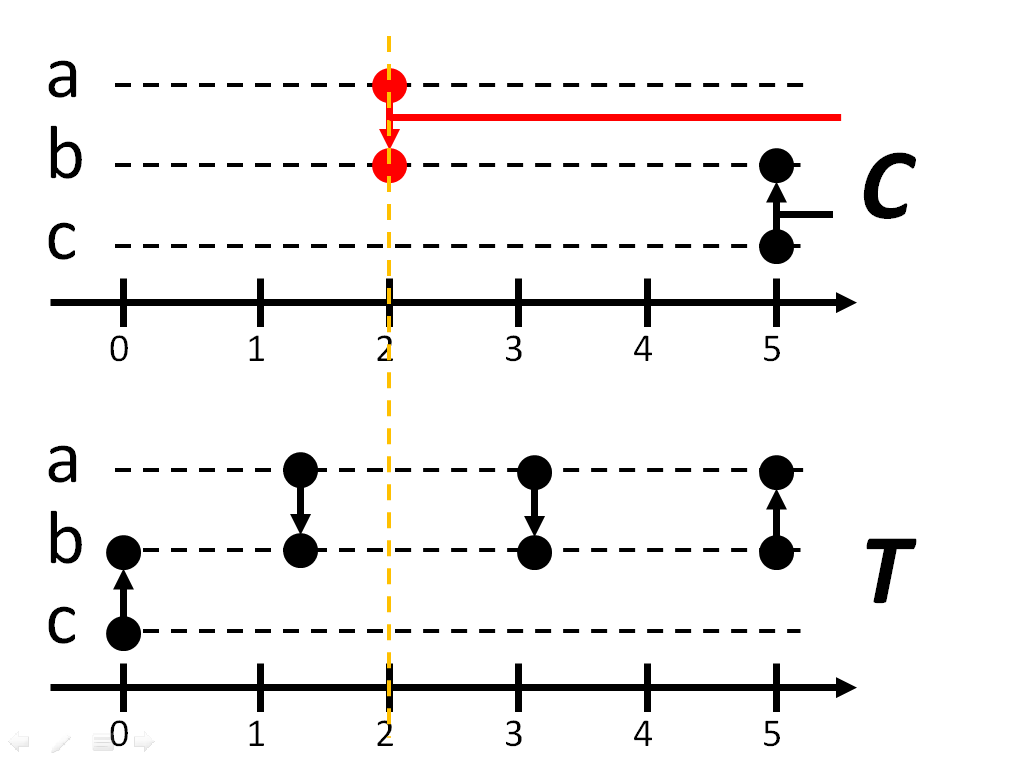
\includegraphics[width=.9\linewidth]{./figures/delta-t-2.png}}
			\only<4>{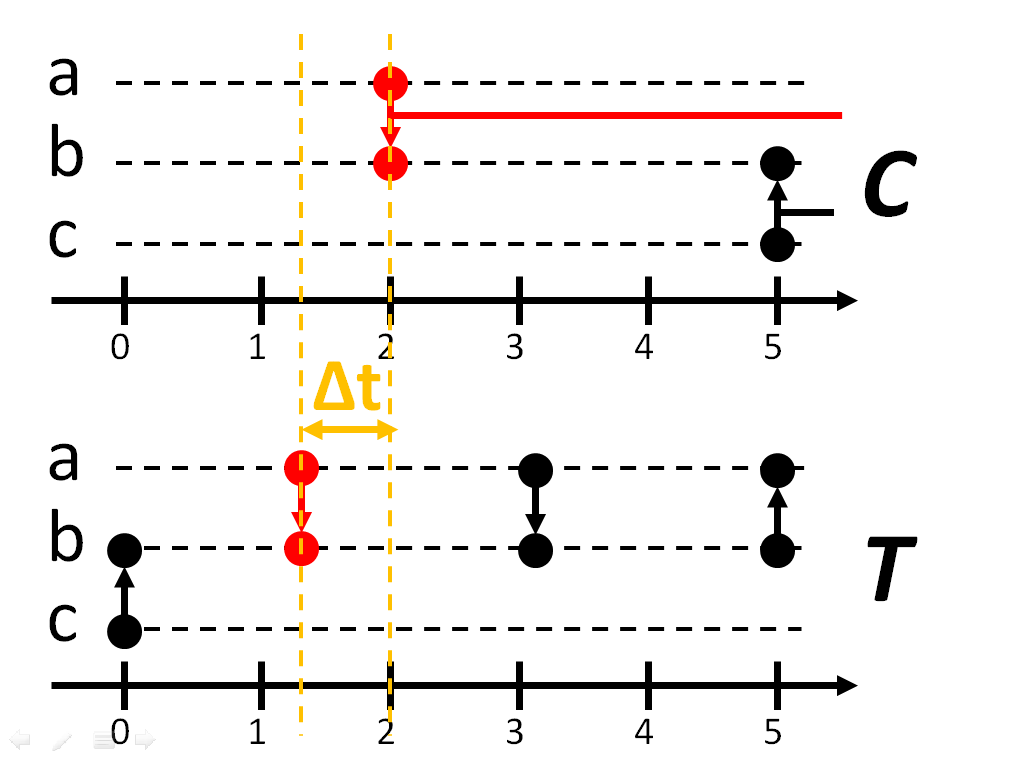
\includegraphics[width=.9\linewidth]{./figures/delta-t-3.png}}
		\end{figure}
	\end{center}
\end{frame}


%------------------------------------------------
	
\begin{frame}
	\frametitle{Time between transactions and certifications - \textbf{Method}}
	\begin{center}
		\begin{figure}
			\only<1>{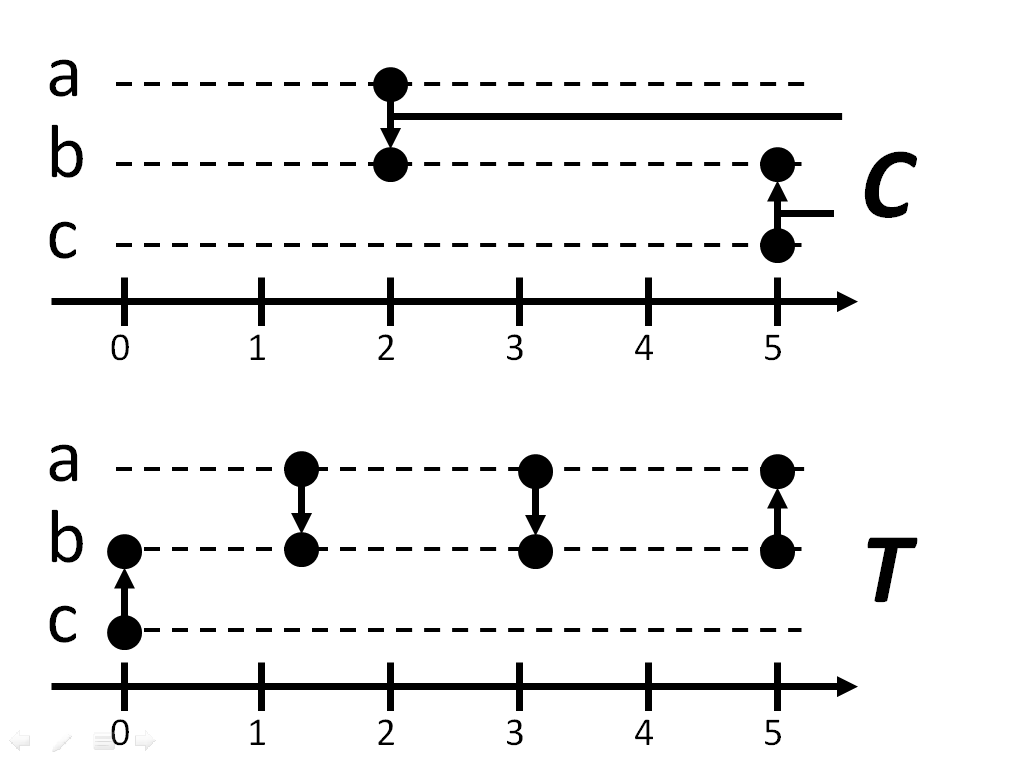
\includegraphics[width=.9\linewidth]{./figures/delta-t-0.png}}
			\only<2>{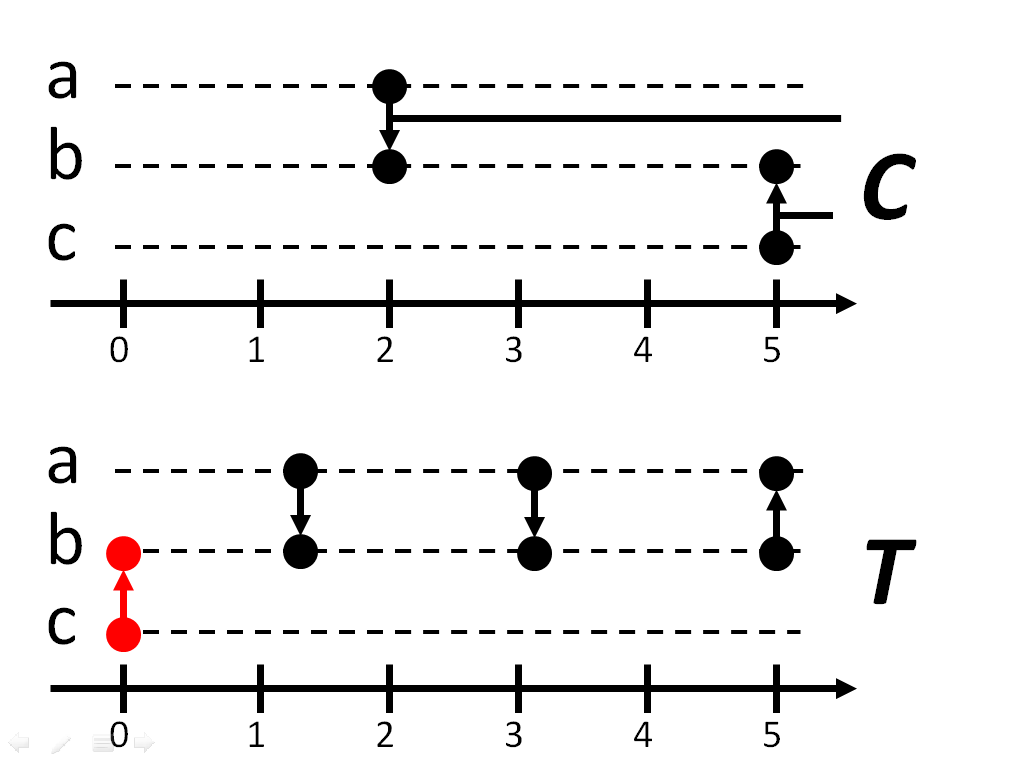
\includegraphics[width=.9\linewidth]{./figures/delta-tt-1.png}}
			\only<3>{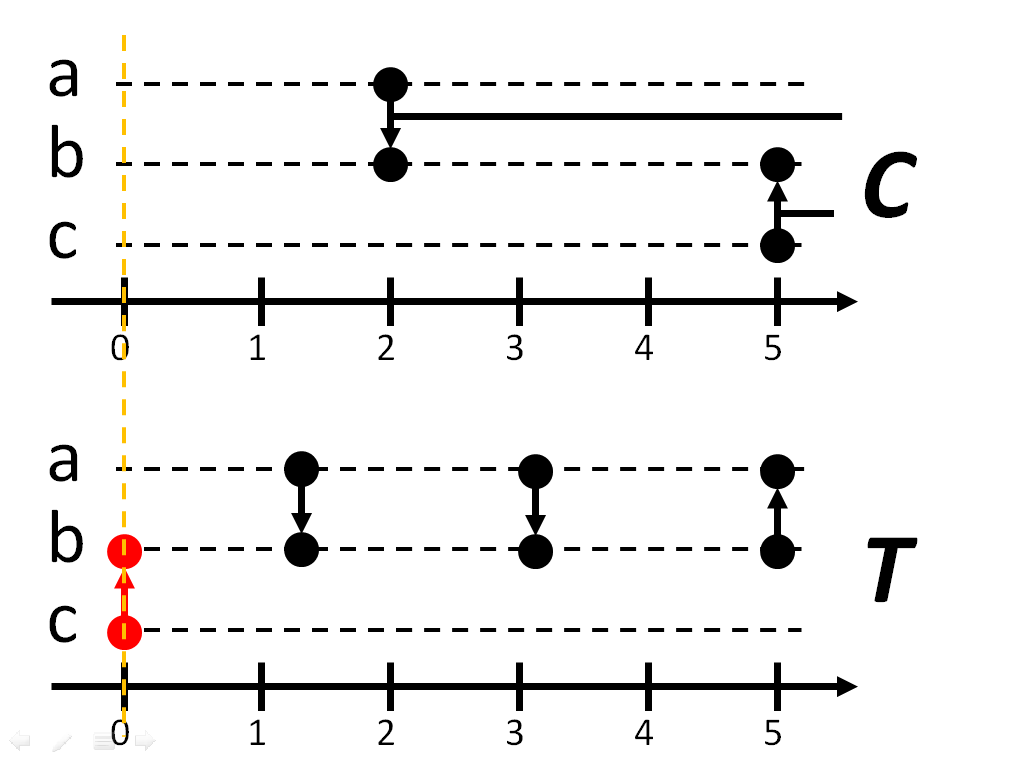
\includegraphics[width=.9\linewidth]{./figures/delta-tt-2.png}}
			\only<4>{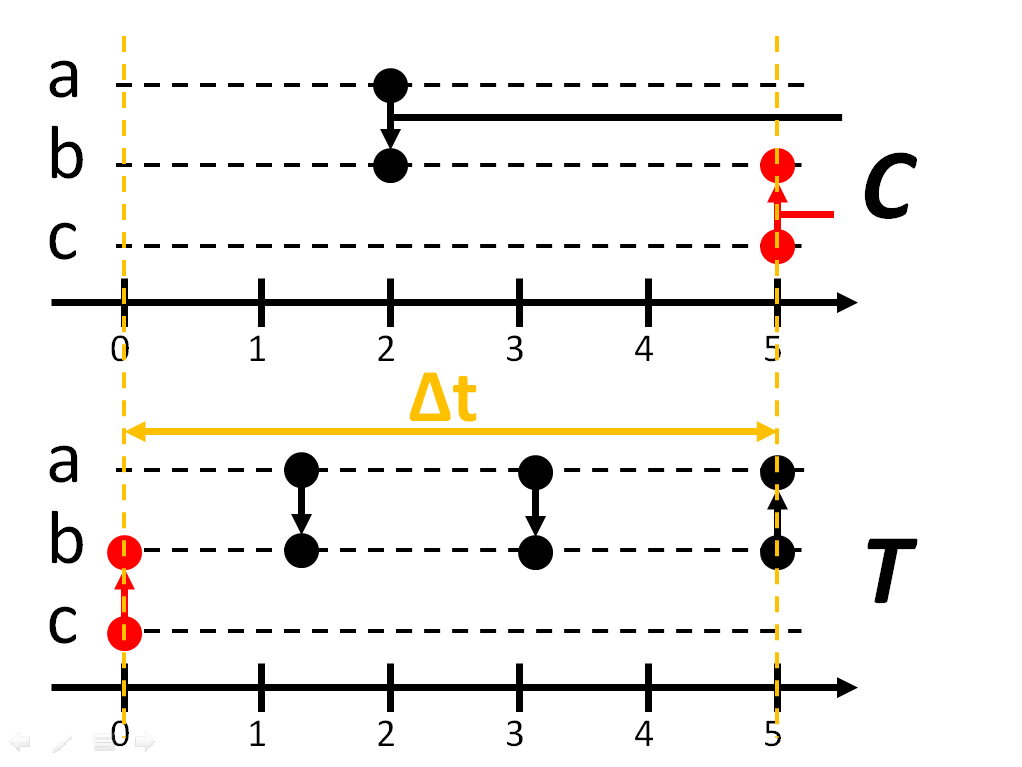
\includegraphics[width=.9\linewidth]{./figures/delta-tt-3.png}}
		\end{figure}
	\end{center}
\end{frame}

%------------------------------------------------

\begin{frame}
	\frametitle{Time between transactions and certifications - \textbf{Results}}
	\begin{figure}
		\only<1>{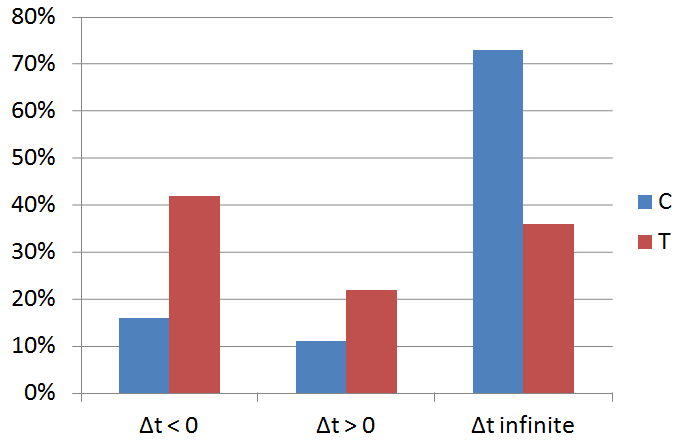
\includegraphics[width=.9\linewidth]{./figures/dt_distri}}
		\only<2>{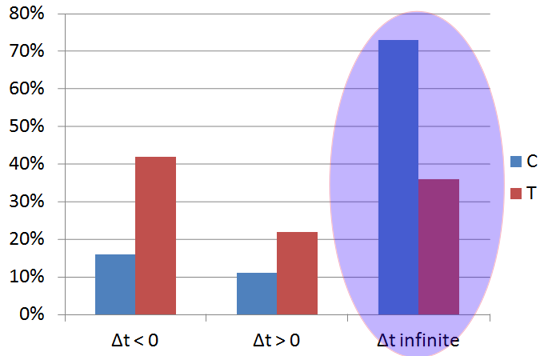
\includegraphics[width=.9\linewidth]{./figures/dt_distri_1}}
		\only<3>{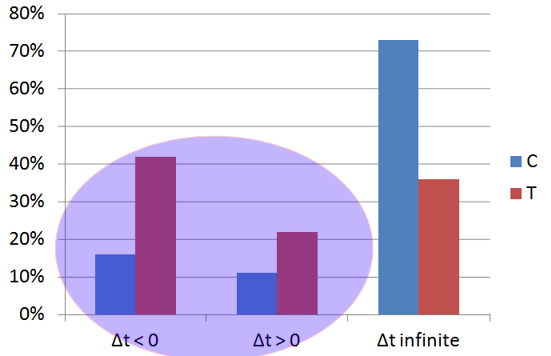
\includegraphics[width=.9\linewidth]{./figures/dt_distri_2}}
	\end{figure}
\end{frame}


%------------------------------------------------

\begin{frame}
	\frametitle{Time between transactions and certifications - \textbf{Results}}
	\begin{figure}
		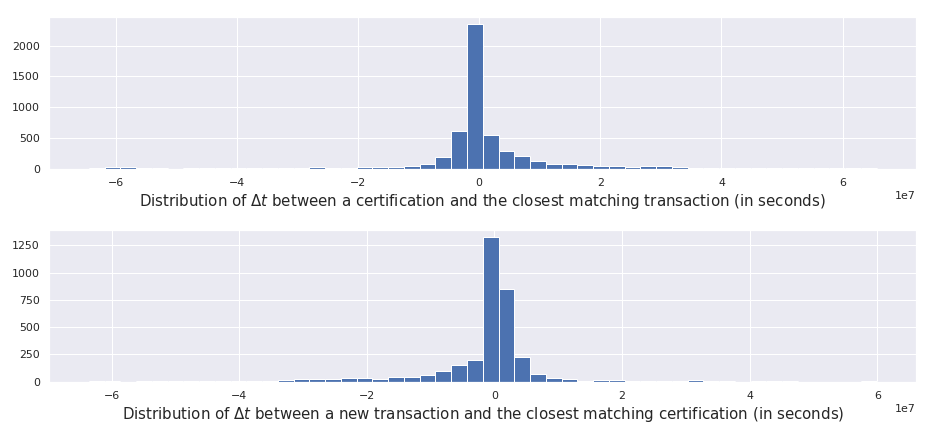
\includegraphics[width=\linewidth]{./figures/delta_t_simple}
	\end{figure}
\end{frame}

%------------------------------------------------
\subsection{Reciprocity and cycles}
%------------------------------------------------

\begin{frame}
	\frametitle{Reciprocity - \textbf{Questions}}
	{\Large \textbf{Questions:}}
	\begin{itemize}
		\item<1-> Are certifications/transactions reciprocal?
		\medskip
		\item<2-> How long does it take to get the opposite certification/transaction?
		\medskip
		\item<3-> How fast is the money cycling?
	\end{itemize}
\end{frame}

%------------------------------------------------

\begin{frame}
	\frametitle{Reciprocity - \textbf{K-Closures} - Ex: 2-closure}
	\begin{center}
		\begin{figure}
			\only<1>{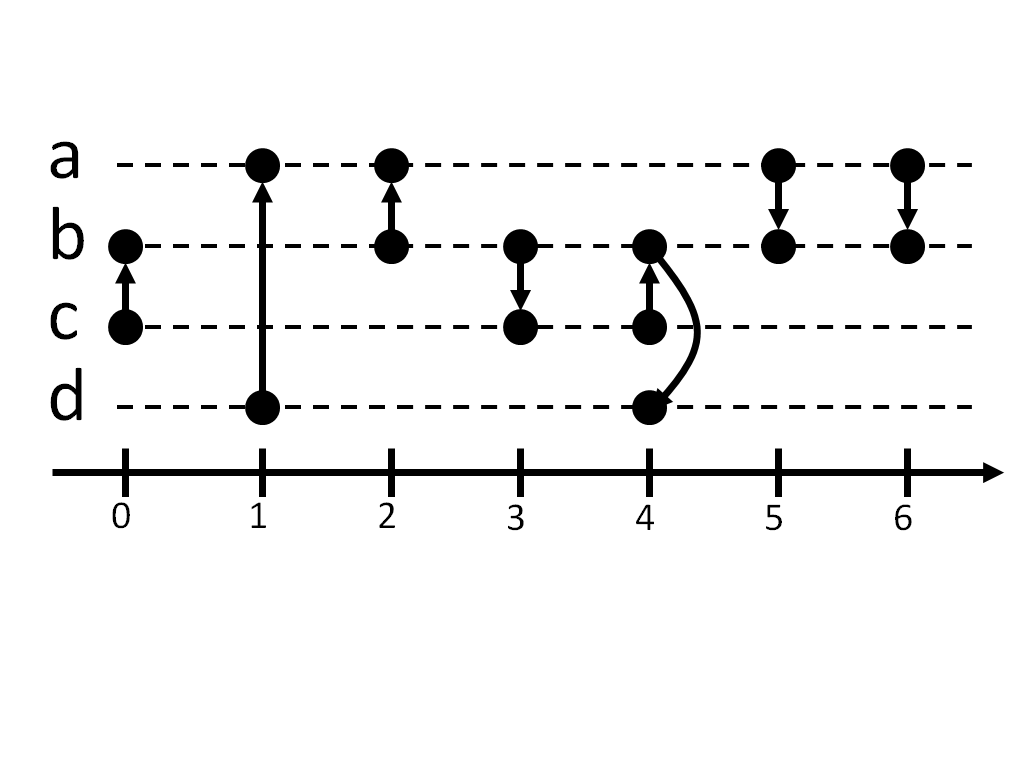
\includegraphics[width=\linewidth]{./figures/2-closure-0}}
			\only<2>{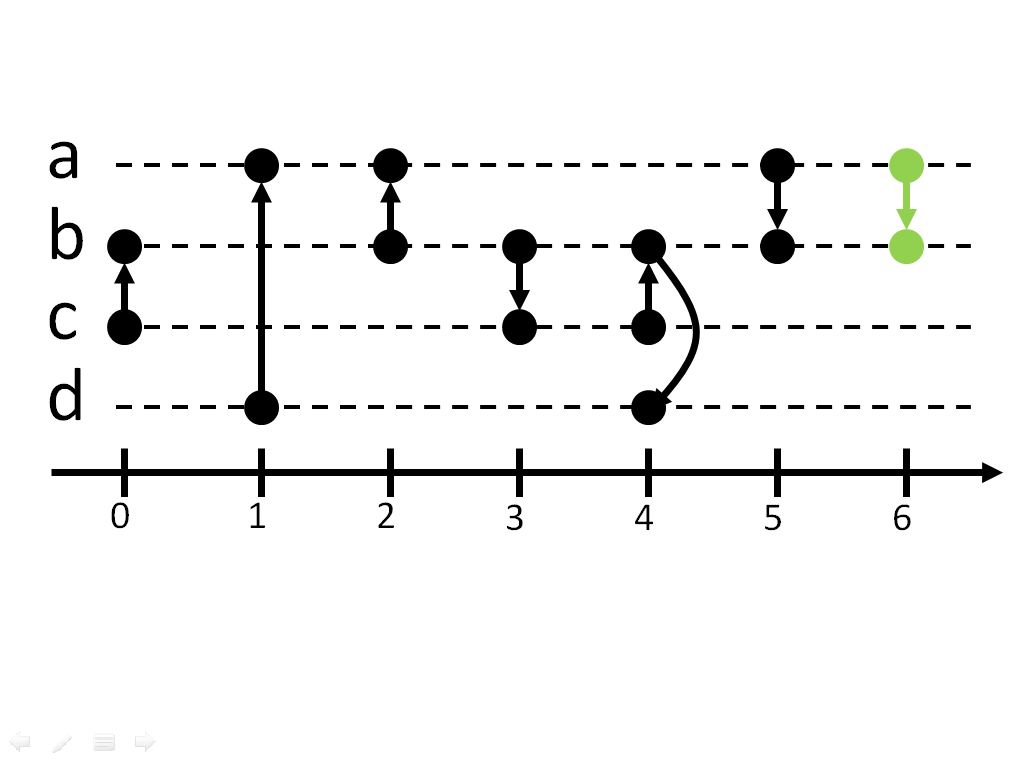
\includegraphics[width=\linewidth]{./figures/2-closure-1}}
			\only<3>{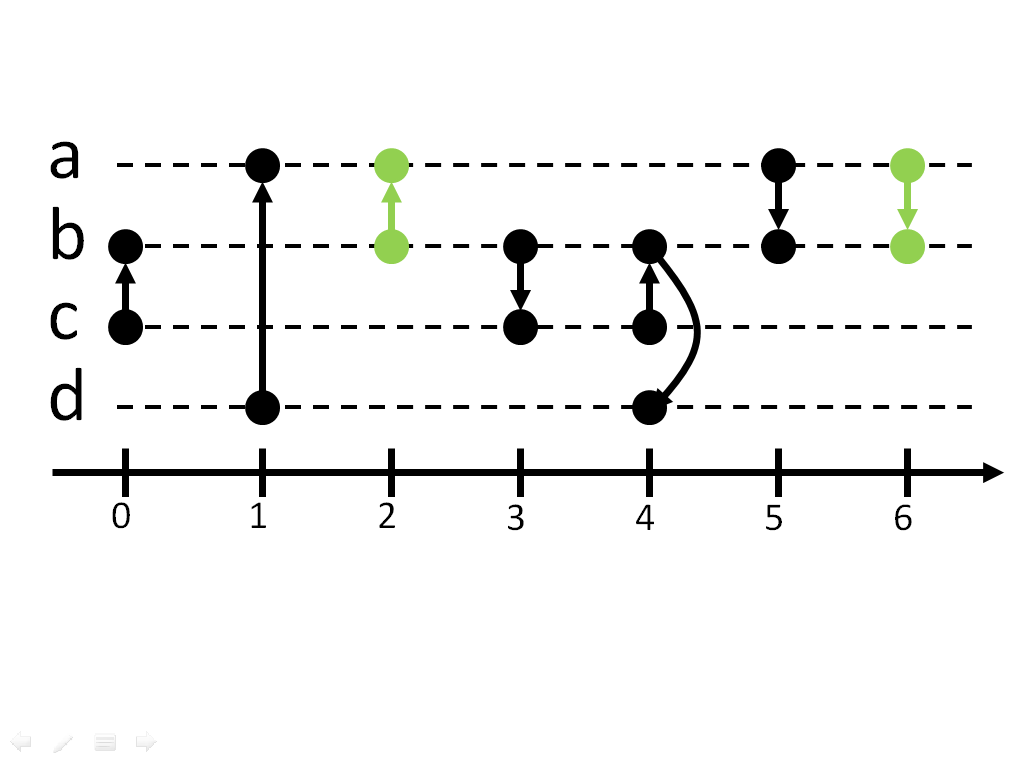
\includegraphics[width=\linewidth]{./figures/2-closure-2}}
			\only<4>{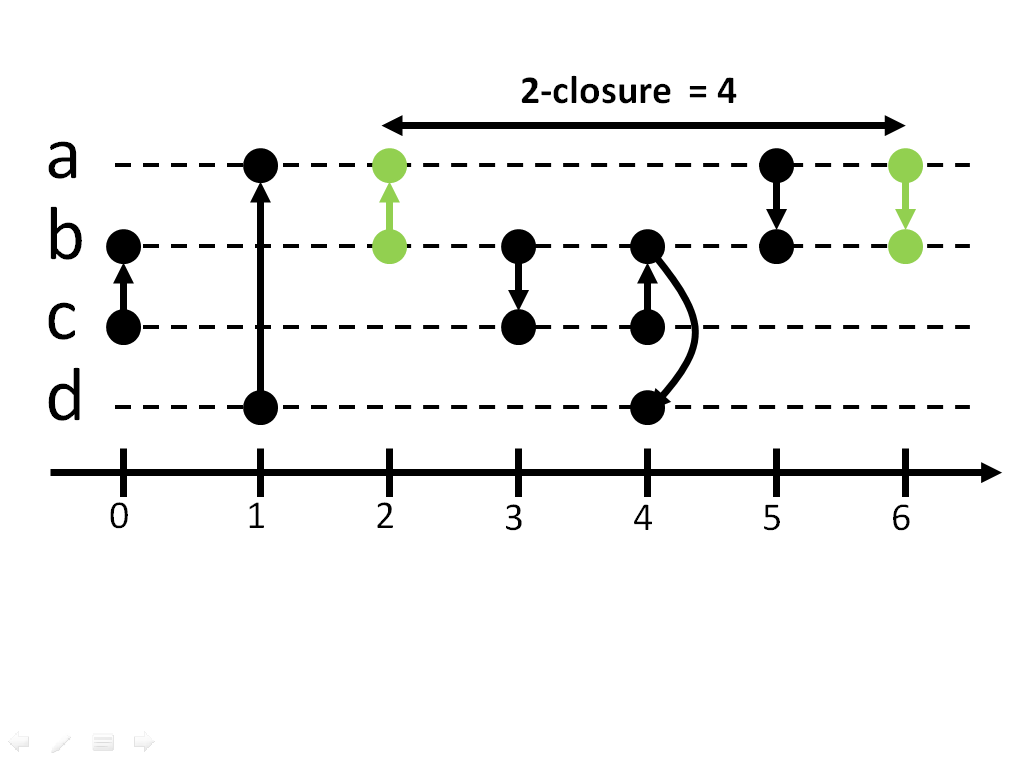
\includegraphics[width=\linewidth]{./figures/2-closure-3}}
		\end{figure}
	\end{center}
\end{frame}

%------------------------------------------------

\begin{frame}
	\frametitle{Reciprocity - \textbf{K-Closures} - Ex: 3-closure}
	\begin{center}
		\begin{figure}
			\only<1>{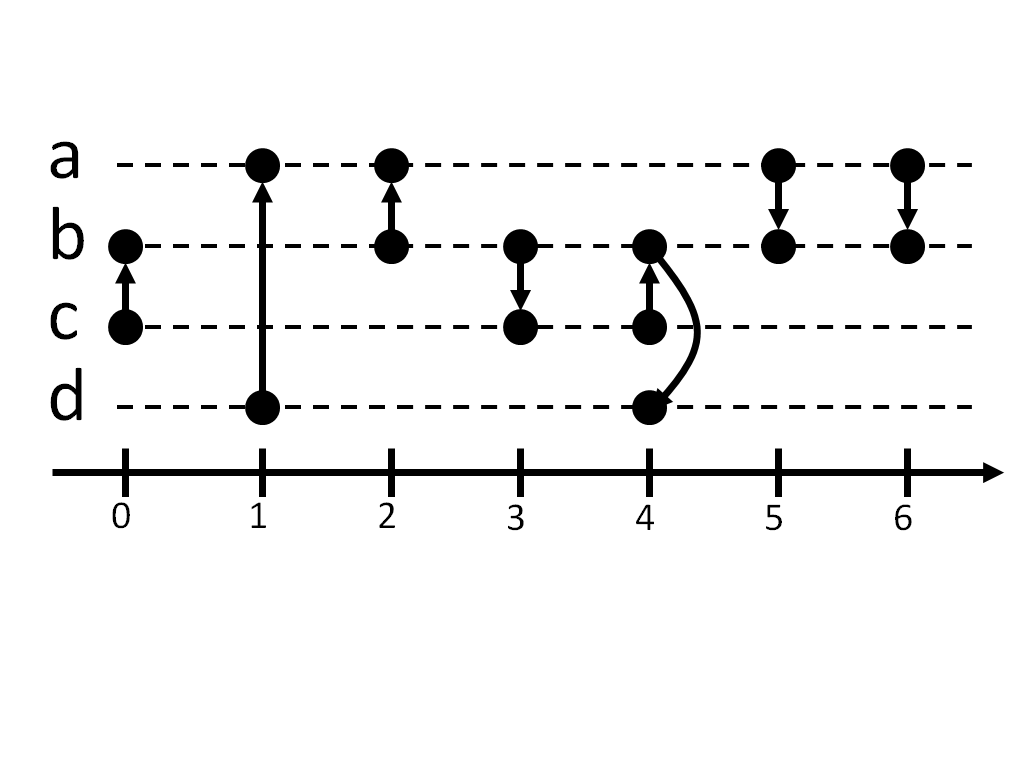
\includegraphics[width=\linewidth]{./figures/2-closure-0}}
			\only<2>{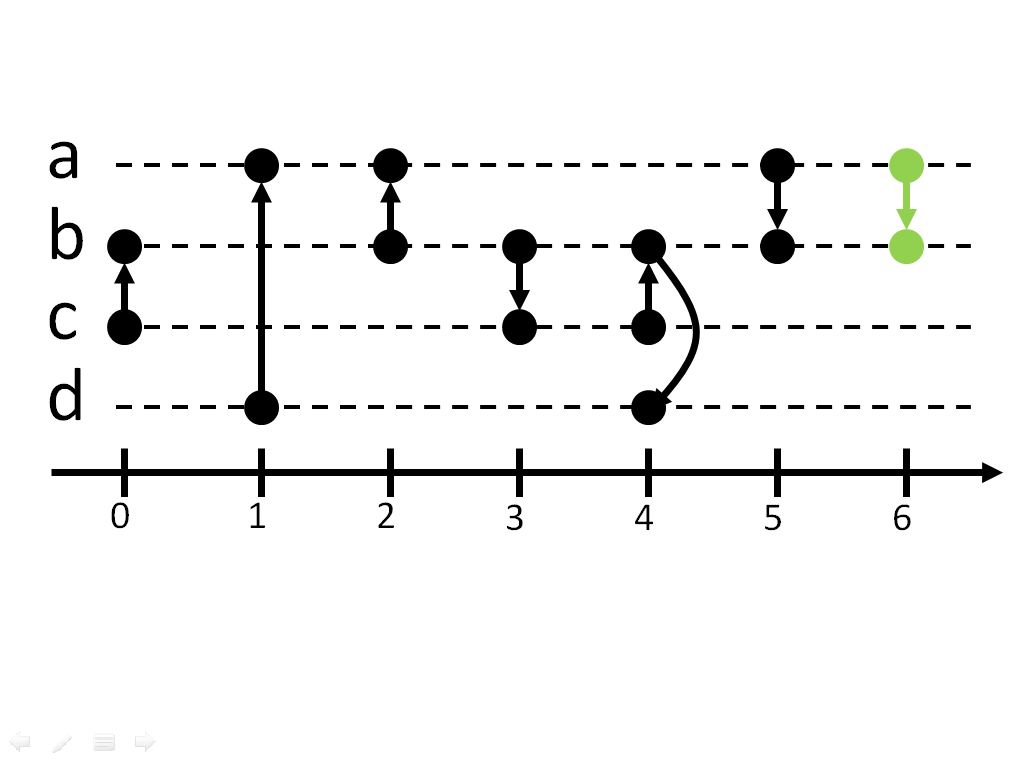
\includegraphics[width=\linewidth]{./figures/2-closure-1}}
			\only<3>{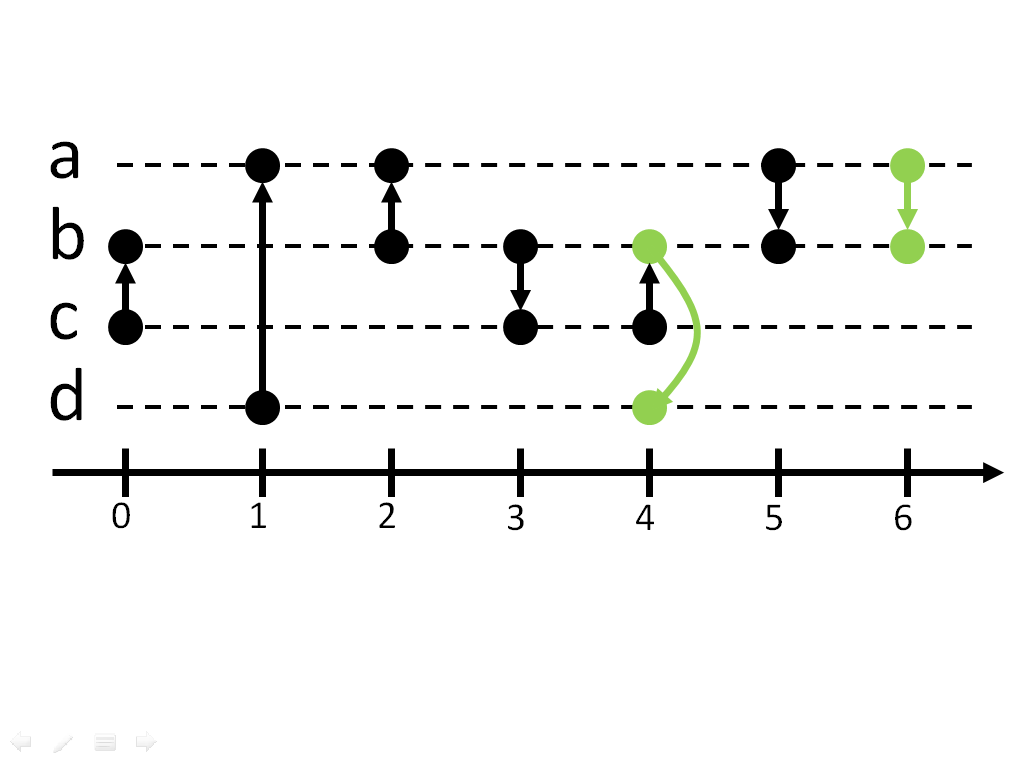
\includegraphics[width=\linewidth]{./figures/3-closure-2}}
			\only<4>{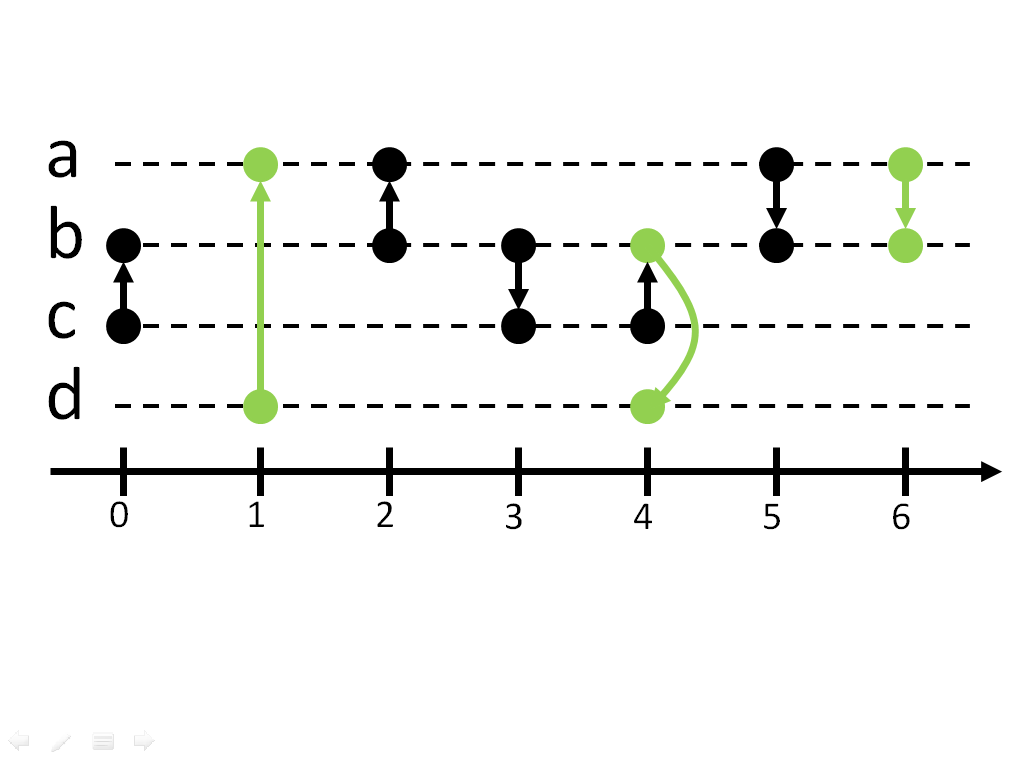
\includegraphics[width=\linewidth]{./figures/3-closure-3}}
			\only<5>{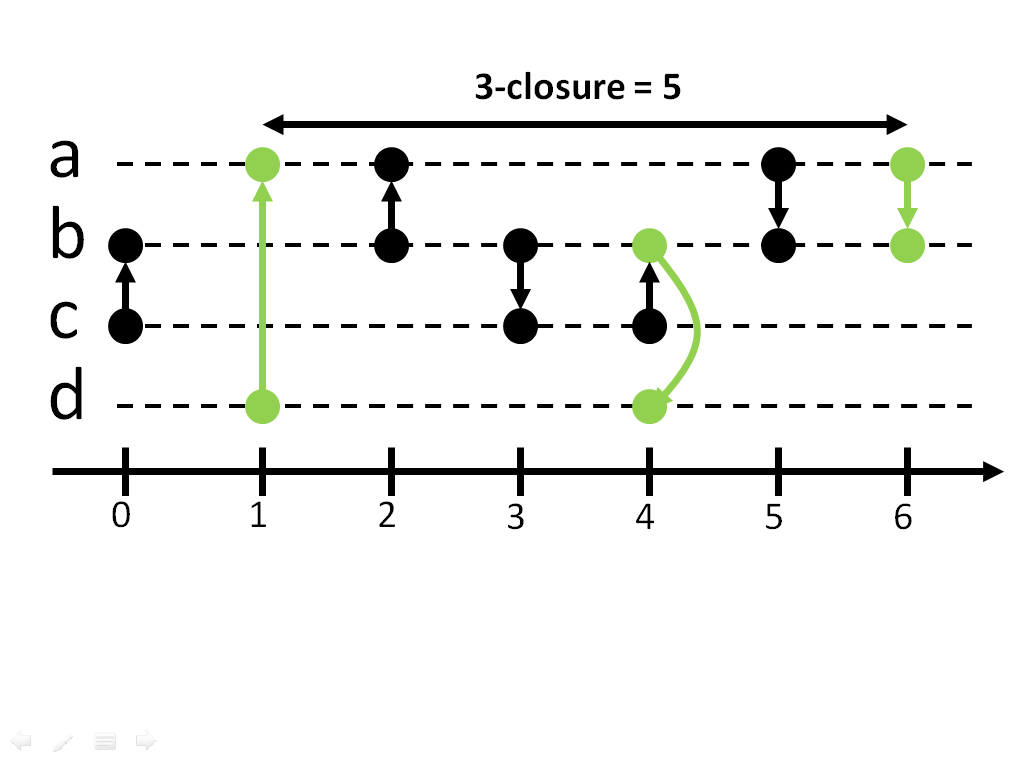
\includegraphics[width=\linewidth]{./figures/3-closure-4}}
		\end{figure}
	\end{center}
\end{frame}

%------------------------------------------------

\begin{frame}
	\frametitle{Reciprocity - \textbf{Results}}
	\begin{figure}
		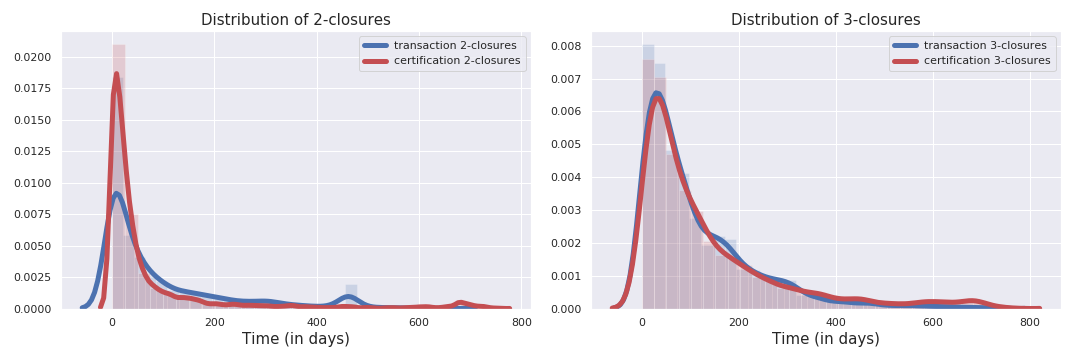
\includegraphics[width=\linewidth]{./figures/2-and-3-closures}
	\end{figure}
\end{frame}

%------------------------------------------------

\begin{frame}
	\Huge{\centerline{Questions?}}
	\bigskip
	{\normalsize Slides available on GitHub: \\ \textit{https://github.com/NicolasGensollen/presentation\_marami\_2019}}
	\bigskip	
	\begin{center}
	{\normalsize \textit{nicolas.gensollen@lip6.fr}}
	\end{center}
\end{frame}

%----------------------------------------------------------------------------------------

\end{document} 